\documentclass[a4paper,12pt]{article}
\usepackage[a4paper,margin=1in]{geometry}
\usepackage{graphicx}
\usepackage{setspace}
\usepackage{titling}
\usepackage{parskip}
\usepackage{lmodern}
\usepackage{subcaption}
\usepackage{caption}
\usepackage[dvipsnames,svgnames,x11names]{xcolor}
\usepackage{float}
\usepackage{amsmath}   
\usepackage{amssymb}
\usepackage[authoryear]{natbib} 
\usepackage[colorlinks=true, citecolor=blue, linkcolor=black, urlcolor=blue]{hyperref}

\begin{document}

\begin{titlepage}
    \centering
    % Logos in corners
    \includegraphics[width=0.4\textwidth]{Cam_logo_bw.png}\\[1.5cm]


    % Title
    {\large \bfseries Disentangling the Components of the Milky Way}\\[0.75cm]
    { \textsc Inferring the Structure of the Milky Way in Phase-Space Using Gaussian Mixture Modelling with Extreme Deconvolution}\\[1.5cm]

    % Author
    \vspace{0.5cm}
    \large
    \textsc{A REPORT PRESENTED}\\[0.3cm]
    \textsc{BY}\\[0.3cm]
    \textsc{RAUNAQ RAI}\\[1cm]

    % Departments
    \normalsize
    \textbf{Departments}\\[0.3cm]
    Department of Physics (Cavendish Laboratory)\\
    Institute of Astronomy\\[1cm]

    % Degree
    \textbf{Degree}\\[0.3cm]
    MPhil in Data Intensive Science\\[1cm]

    % Supervision
    \textbf{Supervision}\\[0.3cm]
    Dr Anke Arentsen\\

    % College Crest and Info
    \vfill
    \includegraphics[width=0.5\textwidth]{St_Edmunds_Logo.png}\\[0.25cm]
    29th June 2025

\end{titlepage}

% -------- CONTENTS PAGE --------
\section*{Abstract}
\newpage

% -------- CONTENTS PAGE --------
\tableofcontents
\newpage

% -------- FIGURES PAGE --------
\listoffigures
\newpage
% -------- TABLES PAGE --------
\listoftables
\newpage

% -------- Introduction --------
\section{Introduction}

The Milky Way Galaxy, host to our solar system, is a spiral galaxy with a centre located approximately 150\,000\,trillion miles (or 25\,000 light\-years) from Earth. Its formation history is complex and remains an active area of research. Being embedded within the Milky Way means we can study it in greate detail than any external galaxy, testing models of galaxy formation with high-precision observational data. One of the central aims of Galactic Archaeology is to reconstruct the Milky Way’s assembly by examining the chemical compositions and dynamical properties of its stars.

In this project, we replicate and extend the analysis of \citet{zhang2024existencemetalpoordiscmilky}, who investigated a very metal-poor disc component in the Milky Way. Very metal poor stars, formed from an interstellar medium unpolluted by earlier generations of supernovae, are among the oldest relics in the Galaxy. Discovering them on disc-like orbits would challenge the conventional view that the disc formed later from already enriched gas \citep{BlandHawthorn2016}, implying instead an earlier onset of disc assembly. Using Gaia DR3, the original study applied a Gaussian Mixture Model with Extreme Deconvolution to the velocity distributions of stars across metallicity bins, probing whether a coherent disc signal persists down to the lowest metallicities.

\subsection{Components of the Milky Way}

The Milky Way is commonly decomposed into four stellar components: a \emph{thin disc}, a \emph{thick disc}, a central \emph{bulge/bar}, and a roughly spherical \emph{halo} \citep{BlandHawthorn2016,Helmi2020}.  
The thin disc dominates, containing $\sim90\%$ of all stars and most of the interstellar gas.  Ongoing star formation is concentrated in the “molecular–gas ring’’ at Galactocentric radii $R\simeq4$–$8\;\mathrm{kpc}$, where young ($\lesssim1\;\mathrm{Gyr}$), metal-rich stars trace nearly circular, co-rotating orbits with low velocity dispersion ($\sigma_\phi \simeq 20\;\mathrm{km\,s^{-1}}$).  
Above the mid-plane lies the thick disc: an older ($\gtrsim8$–$10\;\mathrm{Gyr}$), moderately metal-poor population with $[\mathrm{Fe/H}]\sim-0.6$ to $-1.0$, a scale height of $z_{\mathrm{scale}}\approx1\;\mathrm{kpc}$, and hotter kinematics ($\sigma_z \simeq 40\;\mathrm{km\,s^{-1}}$) while still retaining net prograde rotation.  
Inside $R\lesssim2\;\mathrm{kpc}$, the central bulge—partly bar-shaped—hosts both old, metal-rich stars and a younger, actively forming component; stellar motions there combine bar-driven streaming with high random velocities ($\sigma\sim100\;\mathrm{km\,s^{-1}}$).  
Encasing all of these is the stellar halo, which contributes only a few per cent of the total stellar mass yet harbours the Galaxy’s oldest, most metal-poor stars ($[\mathrm{Fe/H}]\lesssim-1.5$) on highly eccentric or even retrograde orbits.  
Its low density, rich substructure, and extreme kinematics reveal an origin in the hierarchical accretion and tidal disruption of dwarf galaxies and globular clusters.  
Together, the spatial distribution, chemistry, and dynamics of these four components encode the Milky Way’s star-formation history and its sequence of merger events.


\subsection{Metallicity as a Cosmic Clock}

Precise ages for individual old stars are notoriously difficult to measure, so their chemical composition - most commonly the iron-to-hydrogen ratio, $[\mathrm{Fe/H}]$ - is often used as a surrogate clock.  
Very metal-poor (VMP) stars must have formed before successive generations of Type II and Type Ia supernovae had substantially enriched the interstellar medium, and therefore exhibit low $[\mathrm{Fe/H}]$ values.  
Metallicity is inferred spectroscopically from the equivalent widths of metal absorption lines such as Fe \textsc{i} and the Ca \textsc{ii} K line; after correcting for effective temperature and surface gravity, their relative strengths give elemental abundances.
Large surveys (for example APOGEE, GALAH, LAMOST, and the Gaia XP spectra) now provide such measurements for millions of stars, enabling empirical age–metallicity relations that link chemistry to stellar chronometry \citep[e.g.][]{Nordstrom2004,Haywood2013,leung2019deep,Anders2023}.  
These studies consistently show that stars with $[\mathrm{Fe/H}]\lesssim -1$ are typically older than $\sim10$\,Gyr, making low-metallicity populations valuable probes of the Milky Way’s earliest disc-building epochs.


%------------------------------------------------------------------
\subsection{$\Lambda$CDM\,{\rm :} hierarchical growth and a lopsided halo} 
\label{subsec:LCDM_halo}

In the concordance $\Lambda$CDM model, galaxy-sized haloes assemble \emph{hierarchically}:  
small dark-matter clumps form first and then merge to build larger structures.  
Cosmological $N$-body simulations demonstrate that the number of subhaloes of mass $M$ obeys  
$\mathrm{d}n/\mathrm{d}M \propto M^{-1.9}$, a near power-law over many decades in mass  
\citep{Cooper2010,Fall2012}.  
For a Milky-Way–sized halo this translates to  
\begin{itemize}
    \item ${\sim}10^{2}$ \textbf{minor} accretions with $M_{\rm sub}\lesssim10^{9}\,M_\odot$, and 
    \item a few \textbf{major} events with $M_{\rm sub}\gtrsim10^{10}\,M_\odot$
\end{itemize}
over a Hubble time.  

Only a small subset of these haloes ever form appreciable numbers of stars.  
Below a critical virial mass $M_{\rm vir}\!\sim\!10^{11}\,M_\odot$, re-ionisation and stellar feedback
drastically reduce the efficiency of turning gas into stars.  
Consequently, the stellar-mass–halo-mass (SMHM) relation becomes very steep at the low-mass end  
\citep{Purcell2007,BullockBoylanKolchin2017}:  
most low-mass subhaloes are effectively ``dark'', whereas a few relatively massive dwarfs are luminous.  

Hence, while the Milky Way has absorbed \emph{hundreds} of subhaloes,  
\textbf{one or two} of the most massive dwarfs contribute the majority of the halo’s stellar mass;  
the rest add little more than dark matter and dynamical substructure.  
 

Once accreted, dynamical friction drags the most massive satellites deep into the Galactic potential,  
their orbits radialise, and their debris is dispersed throughout the \emph{inner} halo.  
The disrupted stars inherit coherent signatures—high radial anisotropy,  
distinctive angular momenta, and chemically narrow sequences—that survive to the present 
\citep[e.g.][]{HelmiDeZeeuw2000}.  
Consequently, the stellar halo is not a smooth spheroid but a map of the Galaxy’s merger history, 
with the inner halo overwhelmingly shaped by a few dominant progenitors (e.g.\ Gaia–Sausage/Enceladus), 
and the outer halo supplied by many low-mass accretions.

%------------------------------------------------------------------
\subsection{Accretion versus {\it in-situ} disc formation}
\label{subsec:accretion_vs_insitu}

Chemical and kinematic evidence confirms that the metal-poor halo 
is primarily accreted.  The debris of the Gaia–Sausage/Enceladus (GSE) event, for instance, 
is traced by stars with $-2\!<\![\mathrm{Fe/H}]\!<\!-1$ and extreme orbital anisotropy 
($\beta\!\gtrsim\!0.8$; \citealt{Belokurov2018,Helmi2018}).  
At $[\mathrm{Fe/H}]\!\lesssim\!-2$ an even broader mix of minor mergers emerges, 
erasing any global rotation signal \citep{Lancaster2019,Bird2021}.  

Against this backdrop, a number of studies have uncovered stars in the range 
$-2\!<\![\mathrm{Fe/H}]\!<\!-1$ whose velocities resemble a \emph{disc}:  
modest eccentricities and net prograde rotation 
\citep{Norris1985,Chiba2000,Carollo2019,An2020}.  
Gaia has pushed this frontier to $[\mathrm{Fe/H}]\!<\!-2$  
\citep{Sestito2019,Venn2020,Cordoni2020,Mardini2022}.  
Whether these objects represent (i) an {\it in-situ} metal-poor disc or (ii) the spun-up debris of  
earlier mergers remains hotly debated.

%------------------------------------------------------------------
\subsection{Origins of very-metal-poor disc candidates}
\label{subsec:origins_VMP_disc}

Three broad formation scenarios have been proposed:
\begin{enumerate}
    \item \textbf{Early {\it in-situ} disc.}  
          Stars form in a gas-rich disc before $z\!\sim\!4$, and later migrate outward 
          or are dynamically heated; such stars would share the chemistry of the proto-Galaxy. 
    \item \textbf{Proto-galactic building blocks.}  
          VMP stars originate in several massive, gas-rich satellites accreted at high redshift;  
          their debris is dragged into the disc plane as the gaseous disc settles 
          \citep[e.g.][]{Sestito2020}. 
    \item \textbf{Late, minor prograde mergers.}  
          Low-mass satellites on aligned orbits are assimilated after the disc forms,  
          depositing a thin layer of metal-poor stars that retain disc-like kinematics 
          \citep{Santistevan2021}.
\end{enumerate}
Cosmological simulations generally reproduce scenario\;2,  
finding that early mergers dominate the VMP budget while a coherent disc does not appear  
until $z\!\lesssim\!2$ \citep{Gurvich2023}.  

Observationally, \citet{Belokurov2022} identified \textit{Aurora}, a kinematically hot, weakly rotating  
population with $-2\!\lesssim\![\mathrm{Fe/H}]\!\lesssim\!-1.3$, arguing against an extremely early disc.  
Follow-up work shows Aurora to be centrally concentrated \citep{Rix2022,Arentsen2020,Arentsen2020a}, 
consistent with heated debris rather than a long-lived thin disc.  
Furthermore, secular processes such as bar–halo resonances can impart a modest prograde bias to halo stars, 
mimicking a disc signal \citep{Dillamore2023}.  

Unravelling these possibilities demands six-dimensional phase-space information and precision abundances— 
the focus of the present study.

\subsection{This Work}

In this study we assess the claim that the Milky Way hosts a \emph{very-metal-poor} 
(VMP; $[\mathrm{Fe/H}]<-2$) stellar disc.  Our data set is drawn from \textit{Gaia}~DR3, 
which supplies six–dimensional phase–space coordinates—sky position, parallax–based distance, 
proper motions, and radial velocity—for each star, together with homogeneous metallicity and 
$\alpha$-element abundances from the \textit{Gaia} XP pipeline.  To disentangle kinematic 
sub-populations we model, in successive narrow metallicity bins, the full three-dimensional 
velocity distribution $(v_R,v_\phi,v_z)$ with a Gaussian Mixture Model whose parameters are inferred 
via \emph{Extreme Deconvolution}; the XD formalism explicitly folds the individual distance and 
proper-motion uncertainties into the likelihood, ensuring that measurement noise does not bias 
the recovered velocity moments.

Astrophysically, a genuine disc should manifest itself as a high-weight Gaussian centred near the Local 
Standard of Rest ($v_\phi\simeq220\;\mathrm{km\,s^{-1}}$) with small tangential and vertical dispersions 
($\sigma_\phi,\sigma_z\lesssim30\;\mathrm{km\,s^{-1}}$) and negligible mean radial motion, whereas the 
halo or any heated component should appear as a broad, almost isotropic Gaussian with little net rotation 
and dispersions of order $120$–$150\;\mathrm{km\,s^{-1}}$.  By tracking how the weight of the cold, 
rotating component varies with metallicity we can determine when ordered rotation first emerged and 
test whether VMP stars were formed in situ or accreted from a satellite.


% -------- Data --------
\section{Data}

\subsection{Metallicities from \textit{Gaia}\,XP}

Our parent catalogue is the bright ($G<16$) red–giant–branch
sample of \citet{Andrae2023}, who used an
XGBoost\,\footnote{eXtreme Gradient Boosting} regression model
trained on APOGEE\,DR17 and a hand–picked set of very/extremely
metal–poor stars to predict stellar parameters from the
\textit{Gaia}\,DR3 XP spectra.
For each of the 17.6\,million giants the catalogue provides
$[\mathrm{M/H}]$ together with effective temperature and surface gravity; the quoted random uncertainty in
$[\mathrm{M/H}]$ is $\simeq0.1$\,dex for $G\lesssim15$.
Stars with a “high-confidence” metallicity flag
and fall within $-3.5 < [\mathrm{M/H}] < +0.5$ are kept in the sample.

\begin{figure}[h]
  \centering
  %--- Left panel -------------------------------------------------------------
  \begin{subfigure}[b]{0.32\textwidth}
    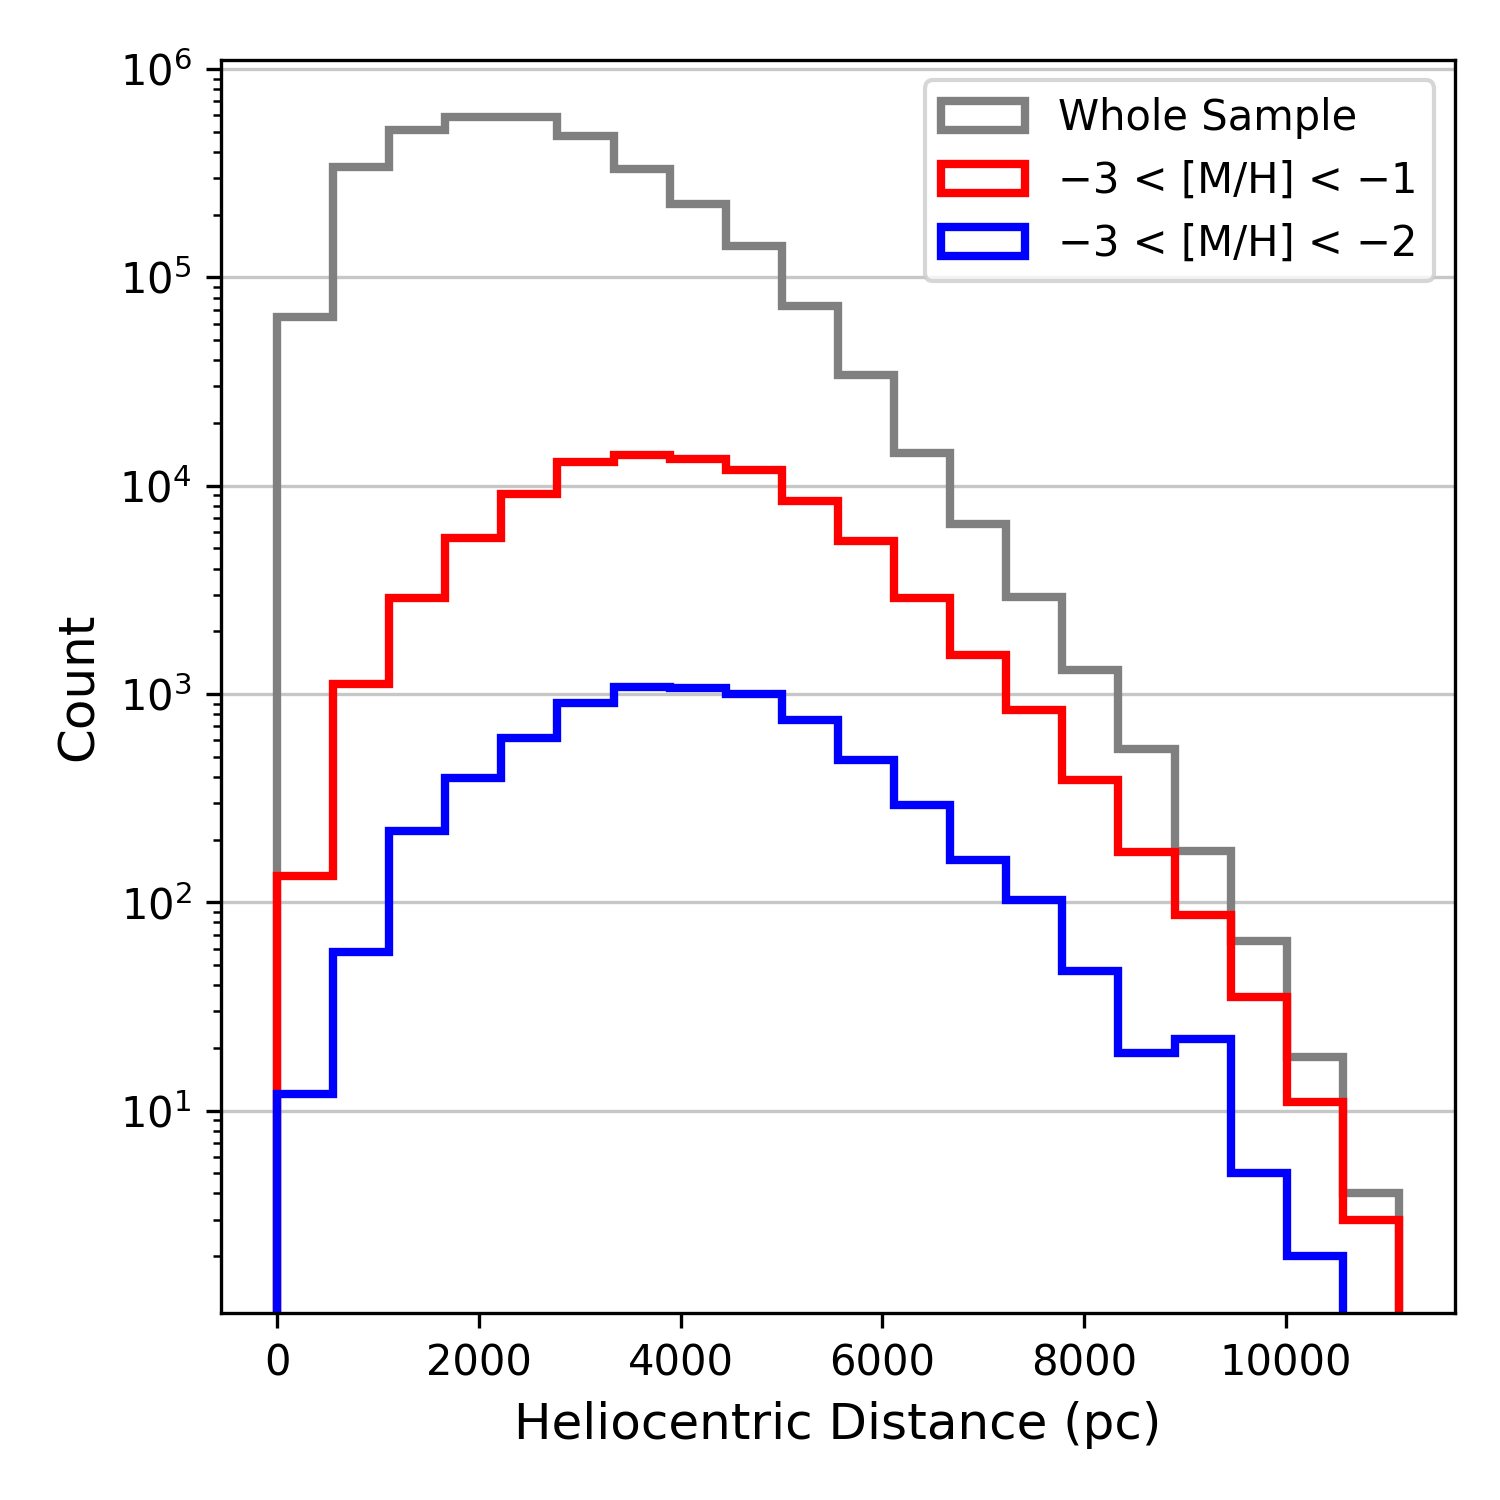
\includegraphics[width=\textwidth]{../figures/distance_histogram.png}
    \caption{Heliocentric distance}
    \label{fig:dist_hist}
  \end{subfigure}\hfill
  %--- Middle panel -----------------------------------------------------------
  \begin{subfigure}[b]{0.32\textwidth}
    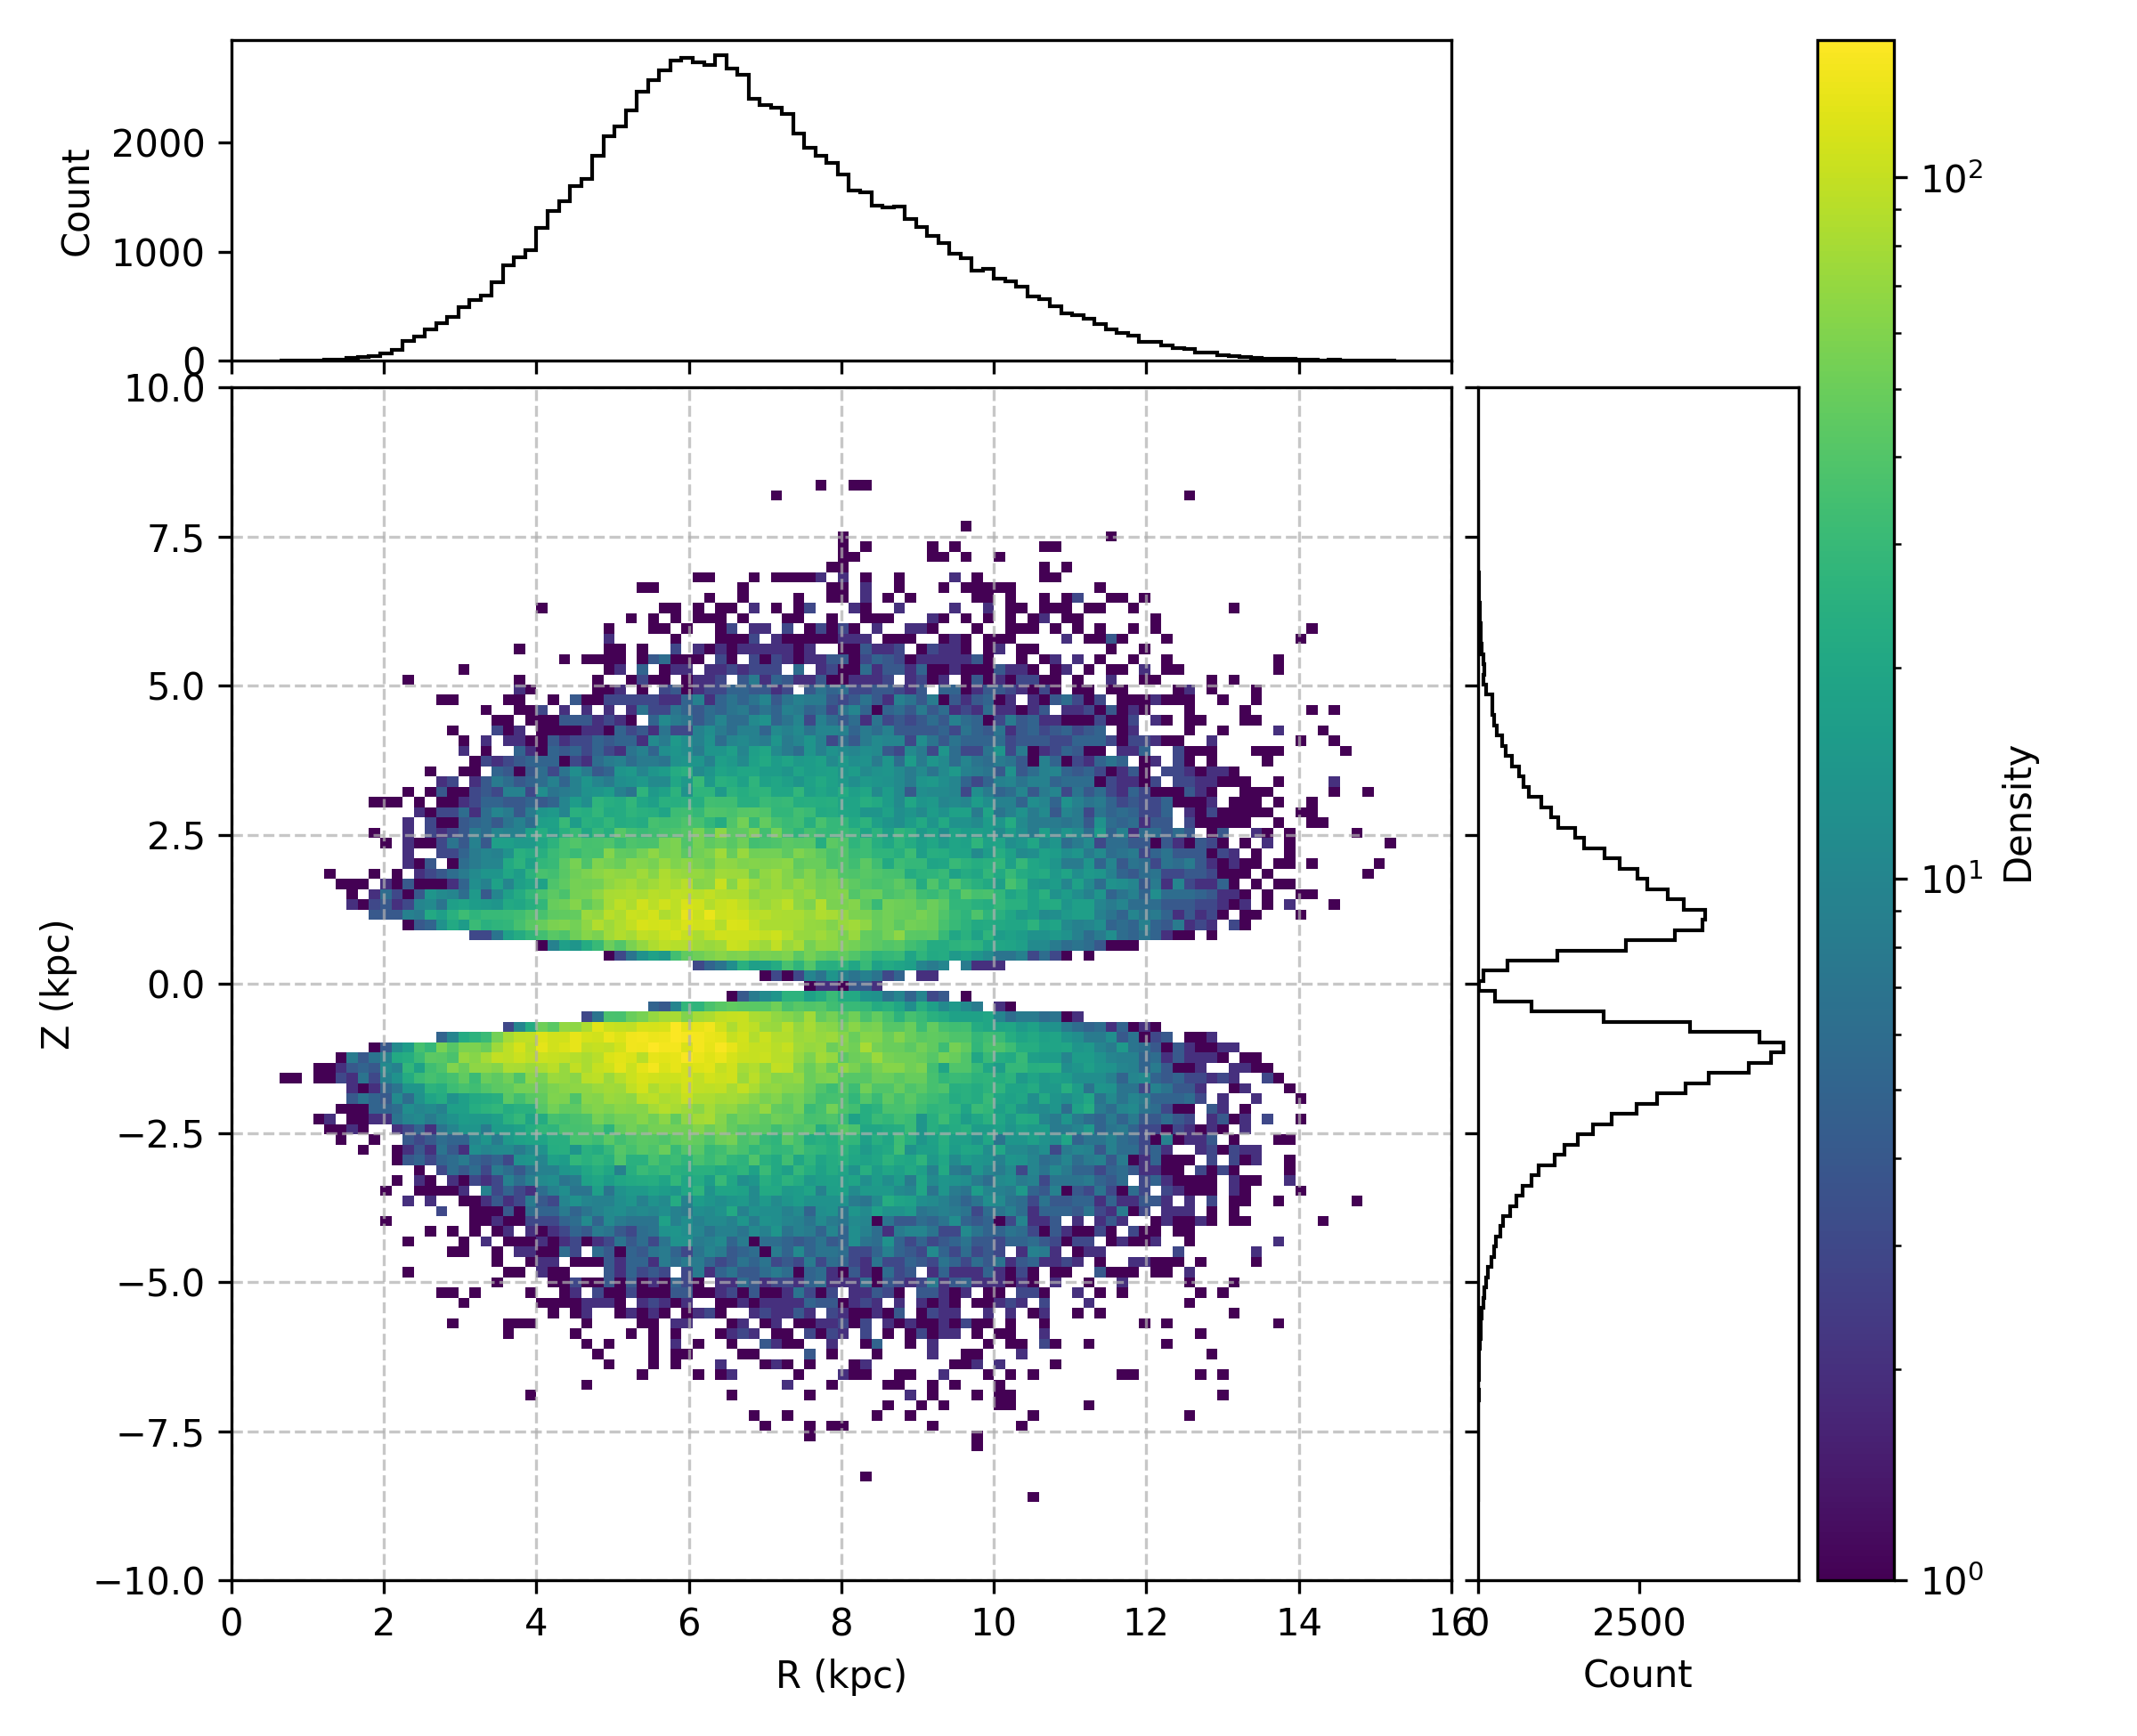
\includegraphics[width=\textwidth]{../figures/ZR_distribution.png}
    \caption{$R$–$Z$ distribution}
    \label{fig:ZR_dist}
  \end{subfigure}\hfill
  %--- Right panel ------------------------------------------------------------
  \begin{subfigure}[b]{0.32\textwidth}
    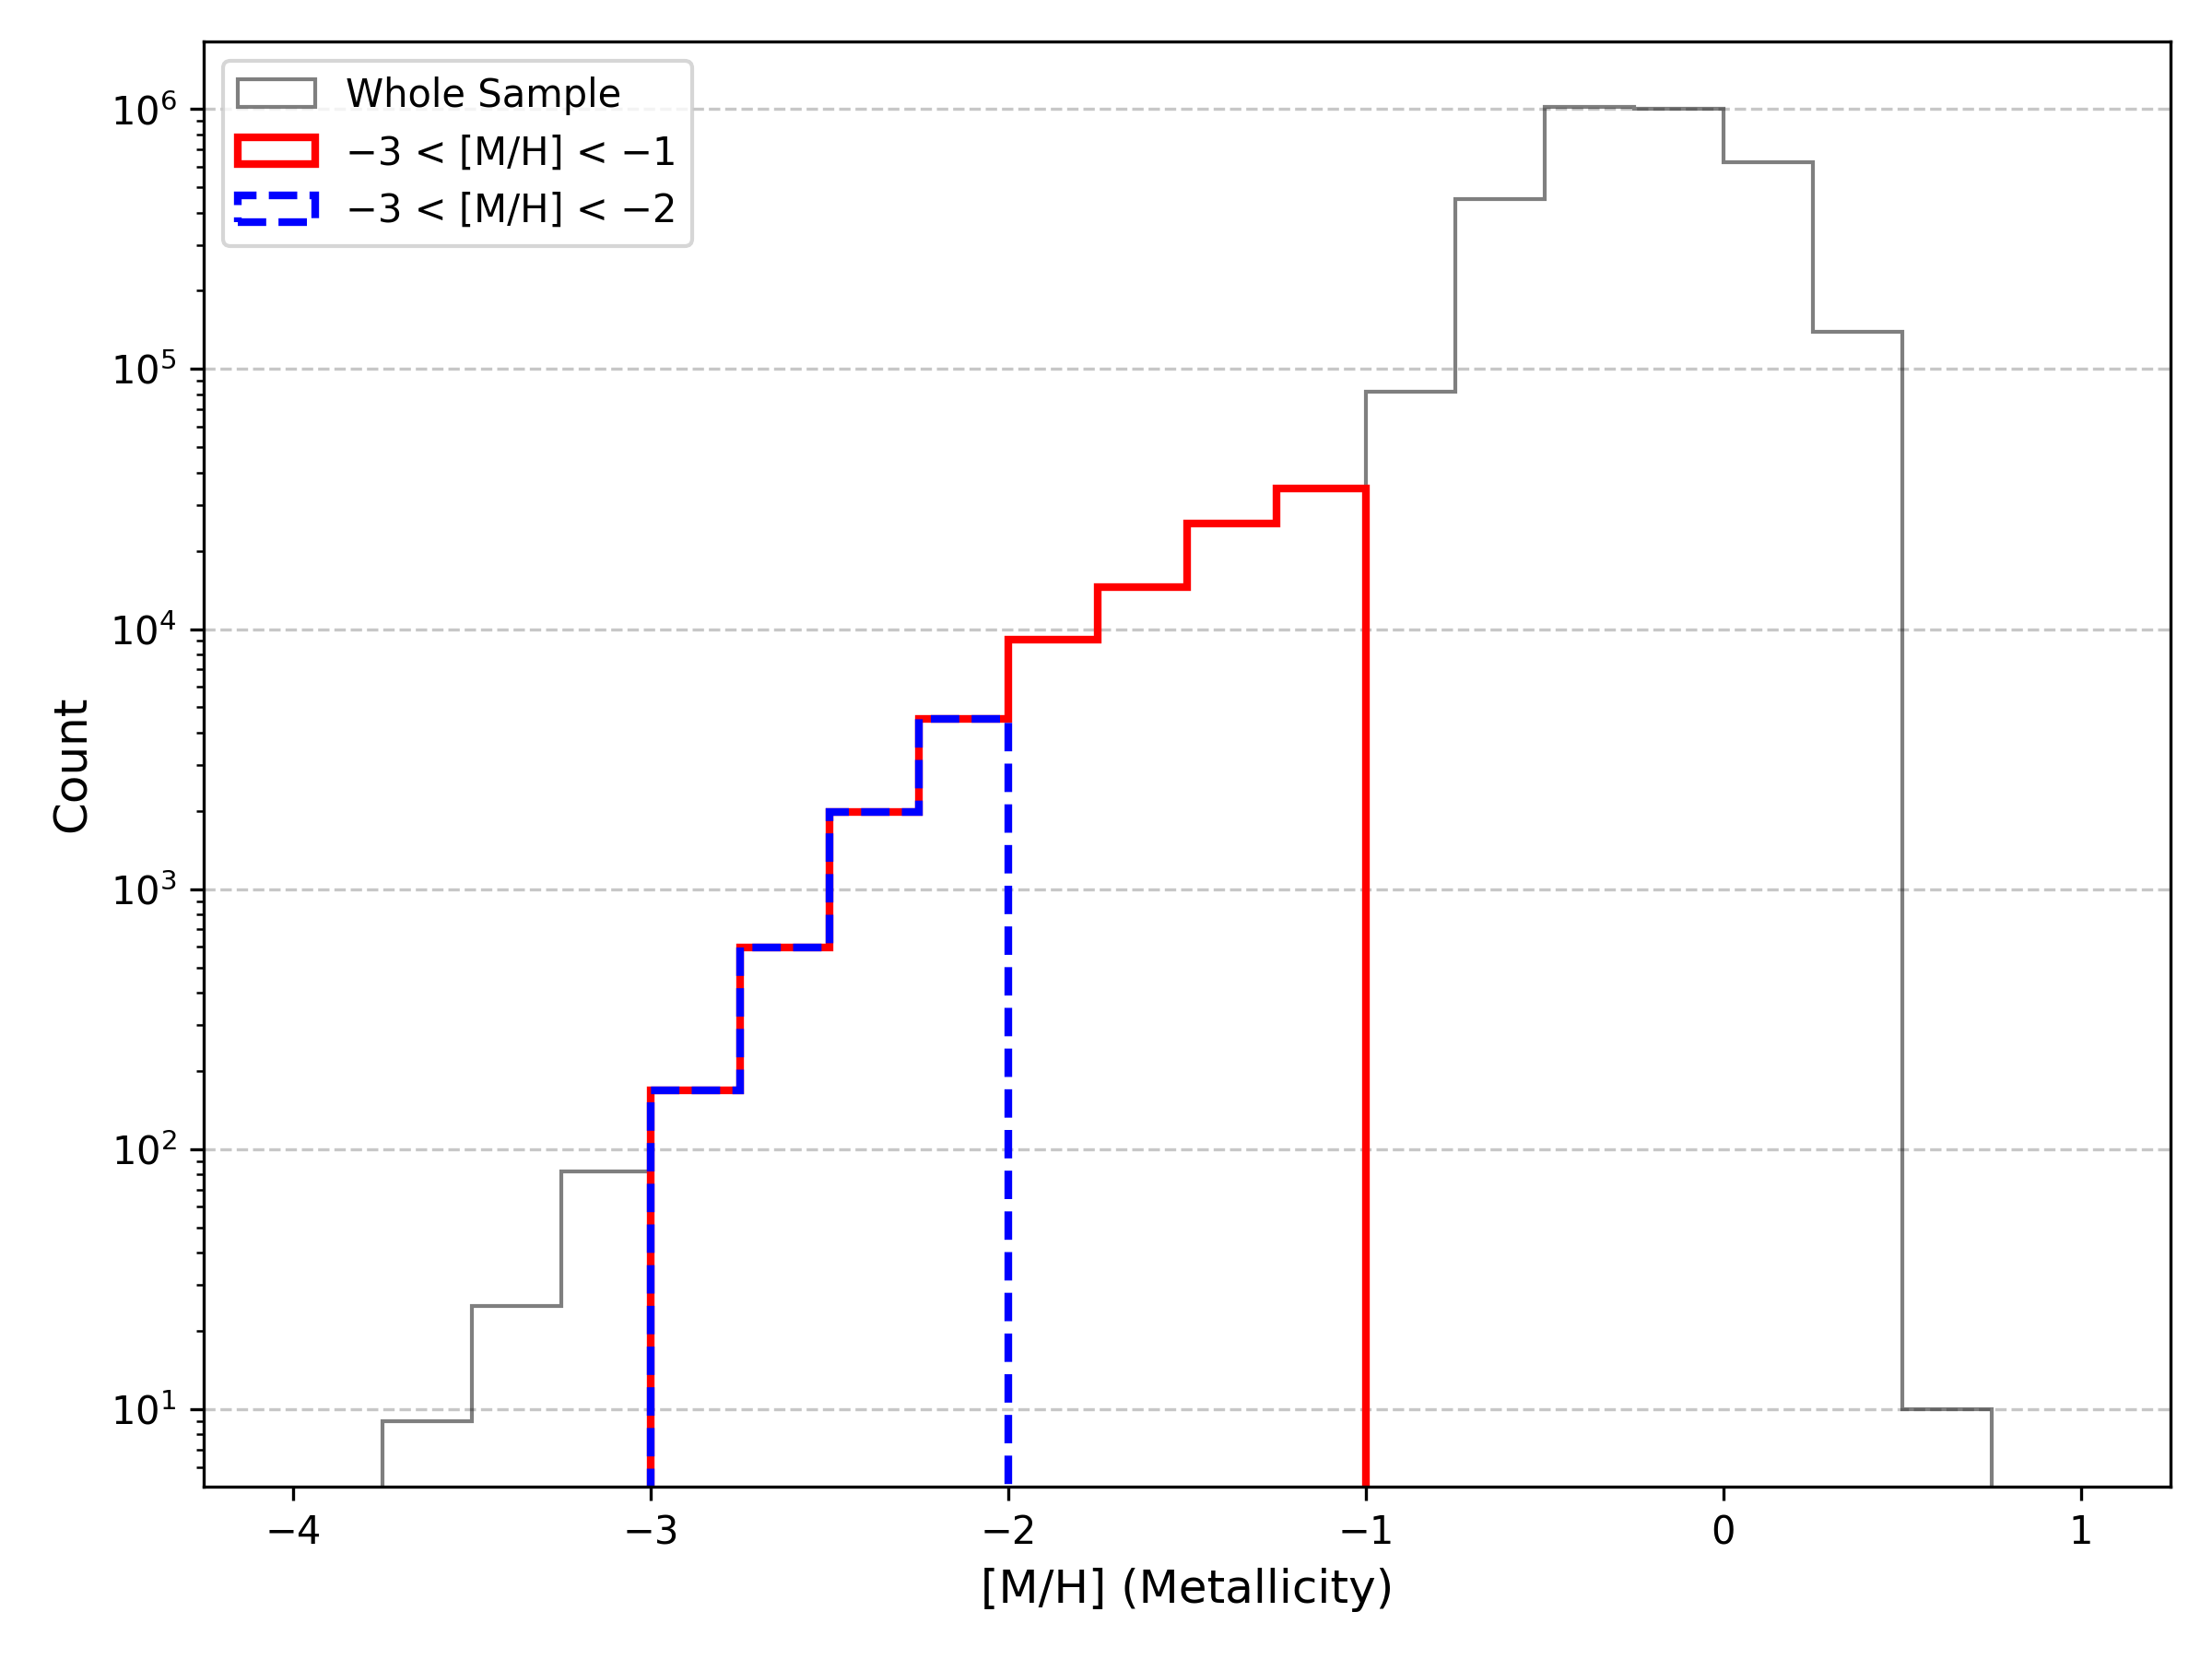
\includegraphics[width=\textwidth]{../figures/metallicity_distribution.png}
    \caption{Metallicity}
    \label{fig:met_dist}
  \end{subfigure}

  \caption{Properties of the final RGB sample after all quality and footprint cuts.
           \textit{Left:} heliocentric-distance histogram for the whole sample (grey); the
           subsets with $-3<\mathrm{[M/H]}<-1$ and $-3<\mathrm{[M/H]}<-2$ are shown in
           solid red and dashed blue, respectively.  
           \textit{Middle:} density map in Galactocentric cylindrical coordinates.  
           The empty band at low $|Z|$ is a selection artefact of our
           latitude/extinction cuts, which deliberately remove the thin–disc mid-plane;
           the concentration around $R\!\simeq\!5$–$8$\,kpc reflects the volume
           accessible to bright RGB stars interior to the Solar circle and coincides
           with the molecular ring region where the stellar surface density peaks.  
           \textit{Right:} Metallicity distribution of our data sample. Line colours are the same as in the left panel.}
  \label{fig:data_properties}
\end{figure}


\subsection{Astrometry, Radial Velocities, and Distances}

Astrometric and spectroscopic measurements are taken from the main
\textit{Gaia}\,DR3 release \citep{GaiaCollaboration2023}, while
heliocentric distances are adopted from the Bayesian photo–geometric
posteriors of \citet{BailerJones2021}.
We impose a conservative fractional–parallax–uncertainty cut
$\sigma_\varpi/\varpi<0.1$ (hereafter \textsc{fpu}) to ensure robust
kinematics and discard objects with \textsc{fpu}$>0.1$.
To mitigate reddening biases in the XP spectra we exclude stars with
$E(B-V)_{\rm SFD}>0.5$ or Galactic latitude $|b|<10^{\circ}$ and mask the
1~deg$^{2}$ regions around known globular clusters and dwarf galaxies \citep{Pace2024}.
After these selections the working sample contains
$\sim$3.4\,million stars.

\subsection{Galactocentric Positions and Velocities}

Six–dimensional phase–space coordinates are obtained with
\texttt{astropy.coordinates}.  We adopt a Galactocentric frame
with $R_{0}=8.1$\,kpc and $Z_{0}=25$\,pc \citep{McMillan2016}, and a solar
velocity\footnote{Cartesian components $(U,V,W)$, where $U$ is radially
outwards, $V$ is aligned with Galactic rotation, and $W$ points to the
North Galactic Pole.}
$(U_{\odot},V_{\odot},W_{\odot})=(11.1,\,245,\,7.25)$\,km\,s$^{-1}$
\citep{Schonrich2010}.
The cylindrical velocity components
$(v_{R},v_{\phi},v_{Z})$ are extracted from the transformed
\texttt{SkyCoord} via the
\texttt{CylindricalRepresentation/CylindricalDifferential} interface.

To propagate measurement errors we generate
$N_{\rm MC}=100$ Monte–Carlo realisations per star, drawing
parallax, proper motions, radial velocity, and distance from their
reported uncertainties (the proper–motion covariance is honoured
through a bivariate normal).  Each realisation is transformed to the
Galactocentric frame, yielding distributions of
$v_{R}$, $v_{\phi}$, and $v_{Z}$; the $1\sigma$ widths of those
distributions are stored as per–star velocity uncertainties.




\begin{figure}[h]
  \centering
  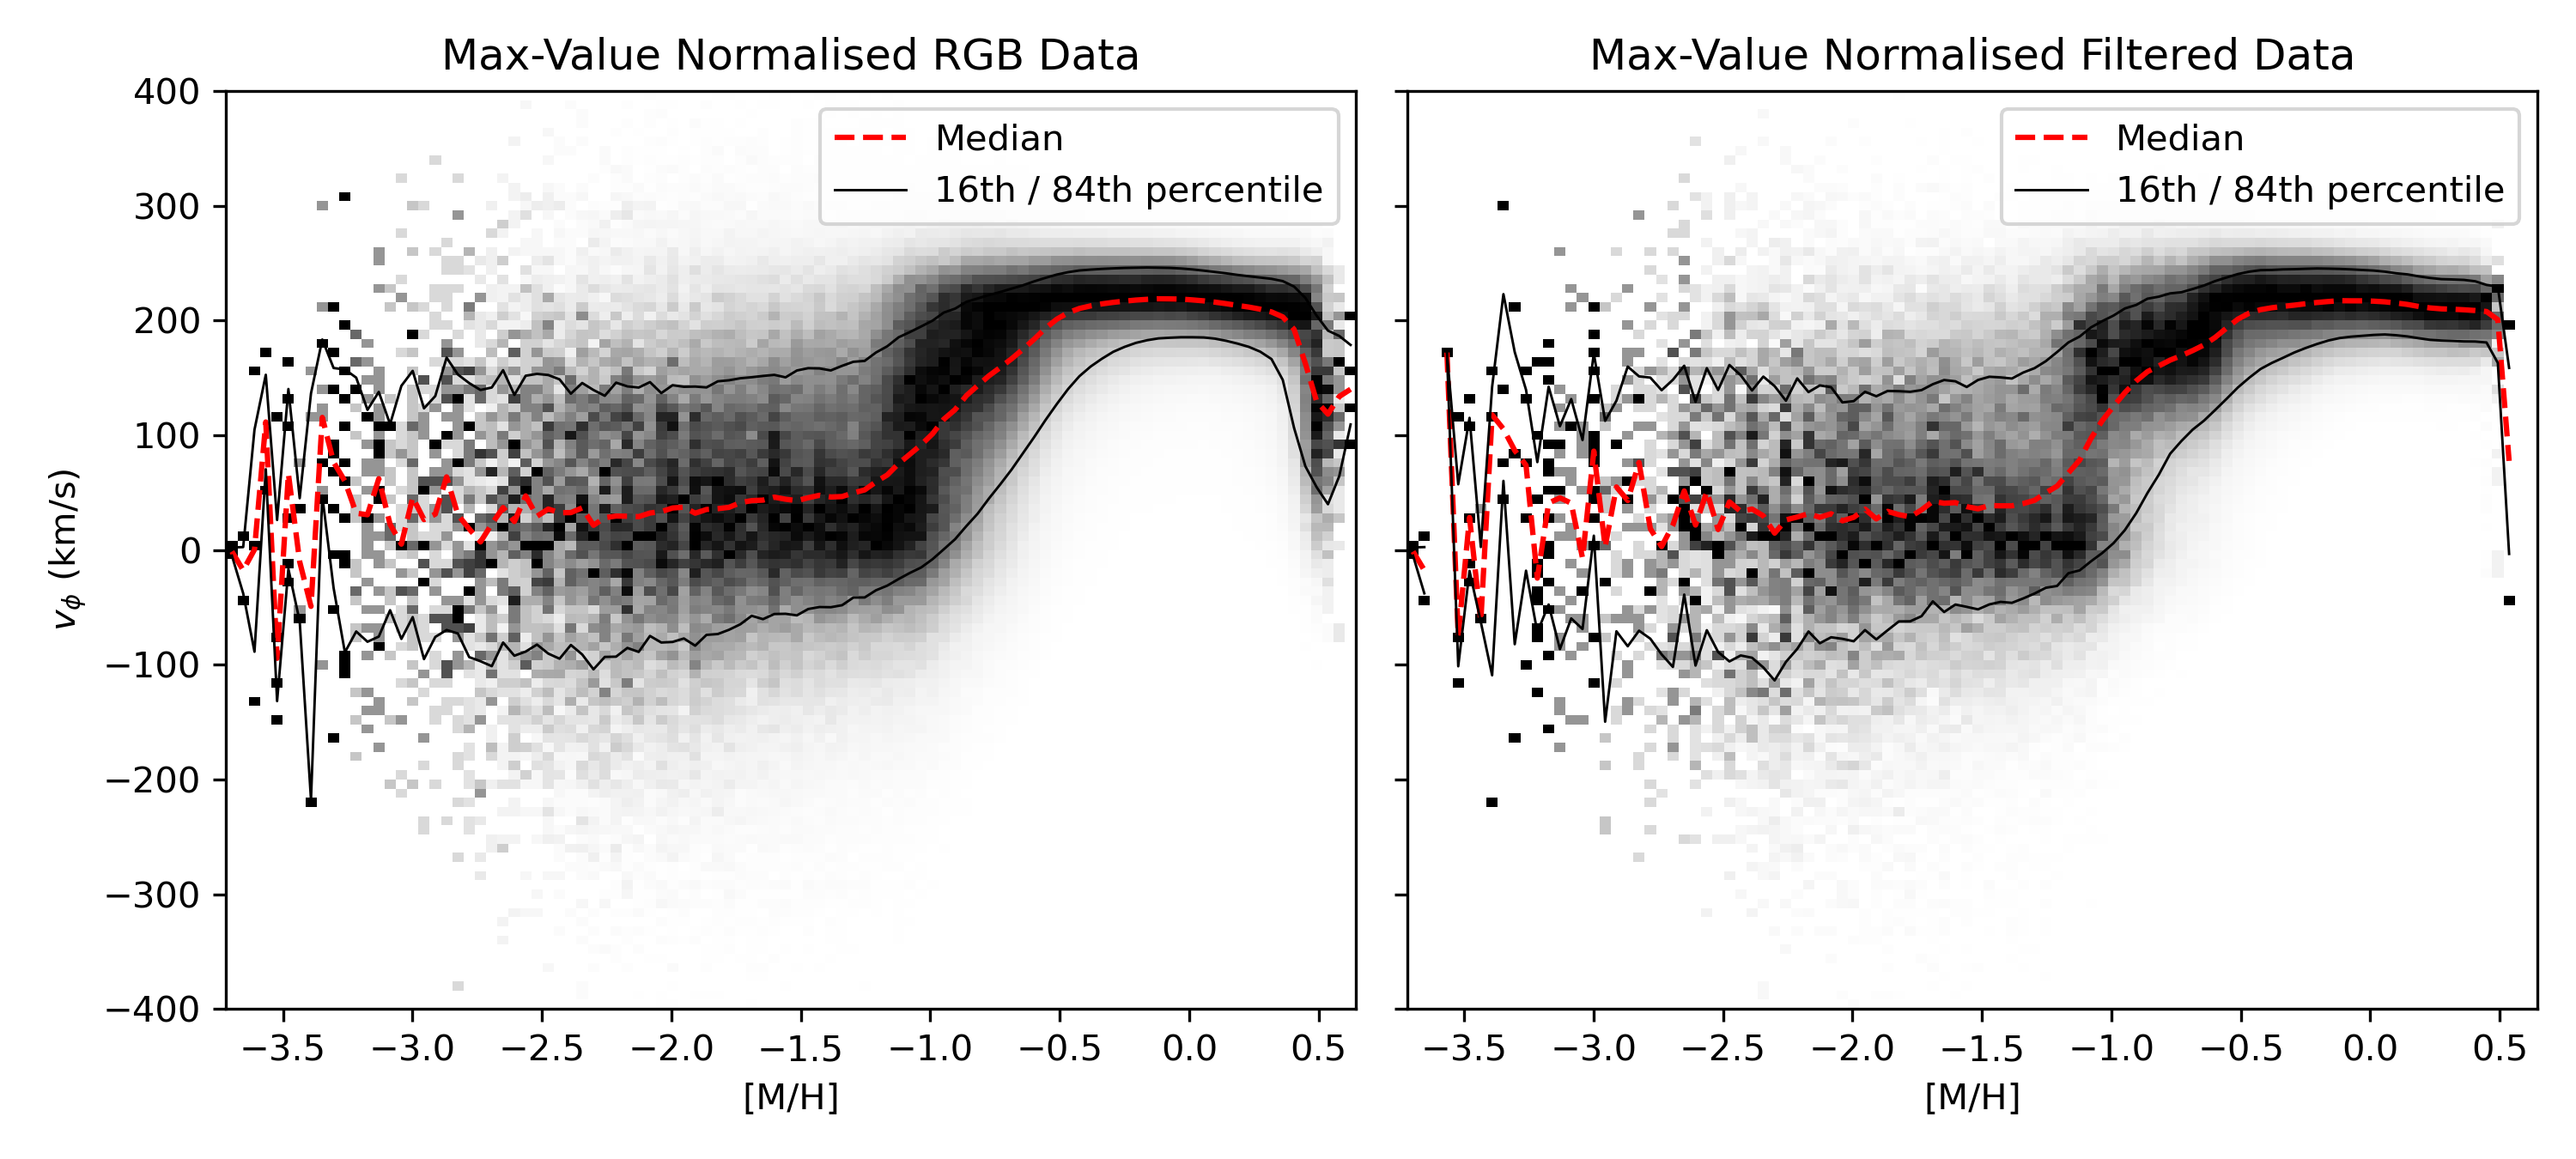
\includegraphics[width=0.94\textwidth]{../figures/vphi_histograms_with_tracks.png}
  \caption{Column-normalised density in the $v_{\phi}$–[M/H] plane.
           \textit{Left:} the bright-RGB catalogue of \citet{Andrae2023}.
           \textit{Right:} the same sample after all distance,
           dust, and quality cuts.  Greyscale pixels show the normalised
           counts in each metallicity bin; the red dashed curve is the
           median $v_{\phi}$, and the black curves trace the 16$^{\text{th}}$
           and 84$^{\text{th}}$ percentiles.}
  \label{fig:vphi_tracks}
\end{figure}


As shown in Figure~\ref{fig:vphi_tracks}, stellar azimuthal velocities
evolve strongly with metallicity.  Halo–like kinematics dominate at
${\rm [M/H]}\lesssim-1.5$\,dex: the median rotation is
$|v_{\phi}|\lesssim 20\;\mathrm{km\;s^{-1}}$ and the
16–84\,percentile span is $\sim120$–$150\;\mathrm{km\;s^{-1}}$,
indicative of a pressure-supported component.  A rapid spin-up
appears at ${\rm [M/H]}\simeq-1.3$\,dex, where the median climbs to
$\sim150\;\mathrm{km\;s^{-1}}$ while the velocity spread contracts.
By ${\rm [M/H]}\gtrsim-0.5$\,dex the median reaches the Local
Standard-of-Rest value ($\approx220\;\mathrm{km\;s^{-1}}$) and the
dispersion falls below $\sim30\;\mathrm{km\;s^{-1}}$, marking the
transition to the present-day thin disc.  Hence the onset of ordered
rotation in the Milky Way occurred when the inter-stellar medium
reached roughly one-tenth solar metallicity, and full kinematic
coldness was achieved only after it became near-solar.


\begin{figure}[h]
  \centering
  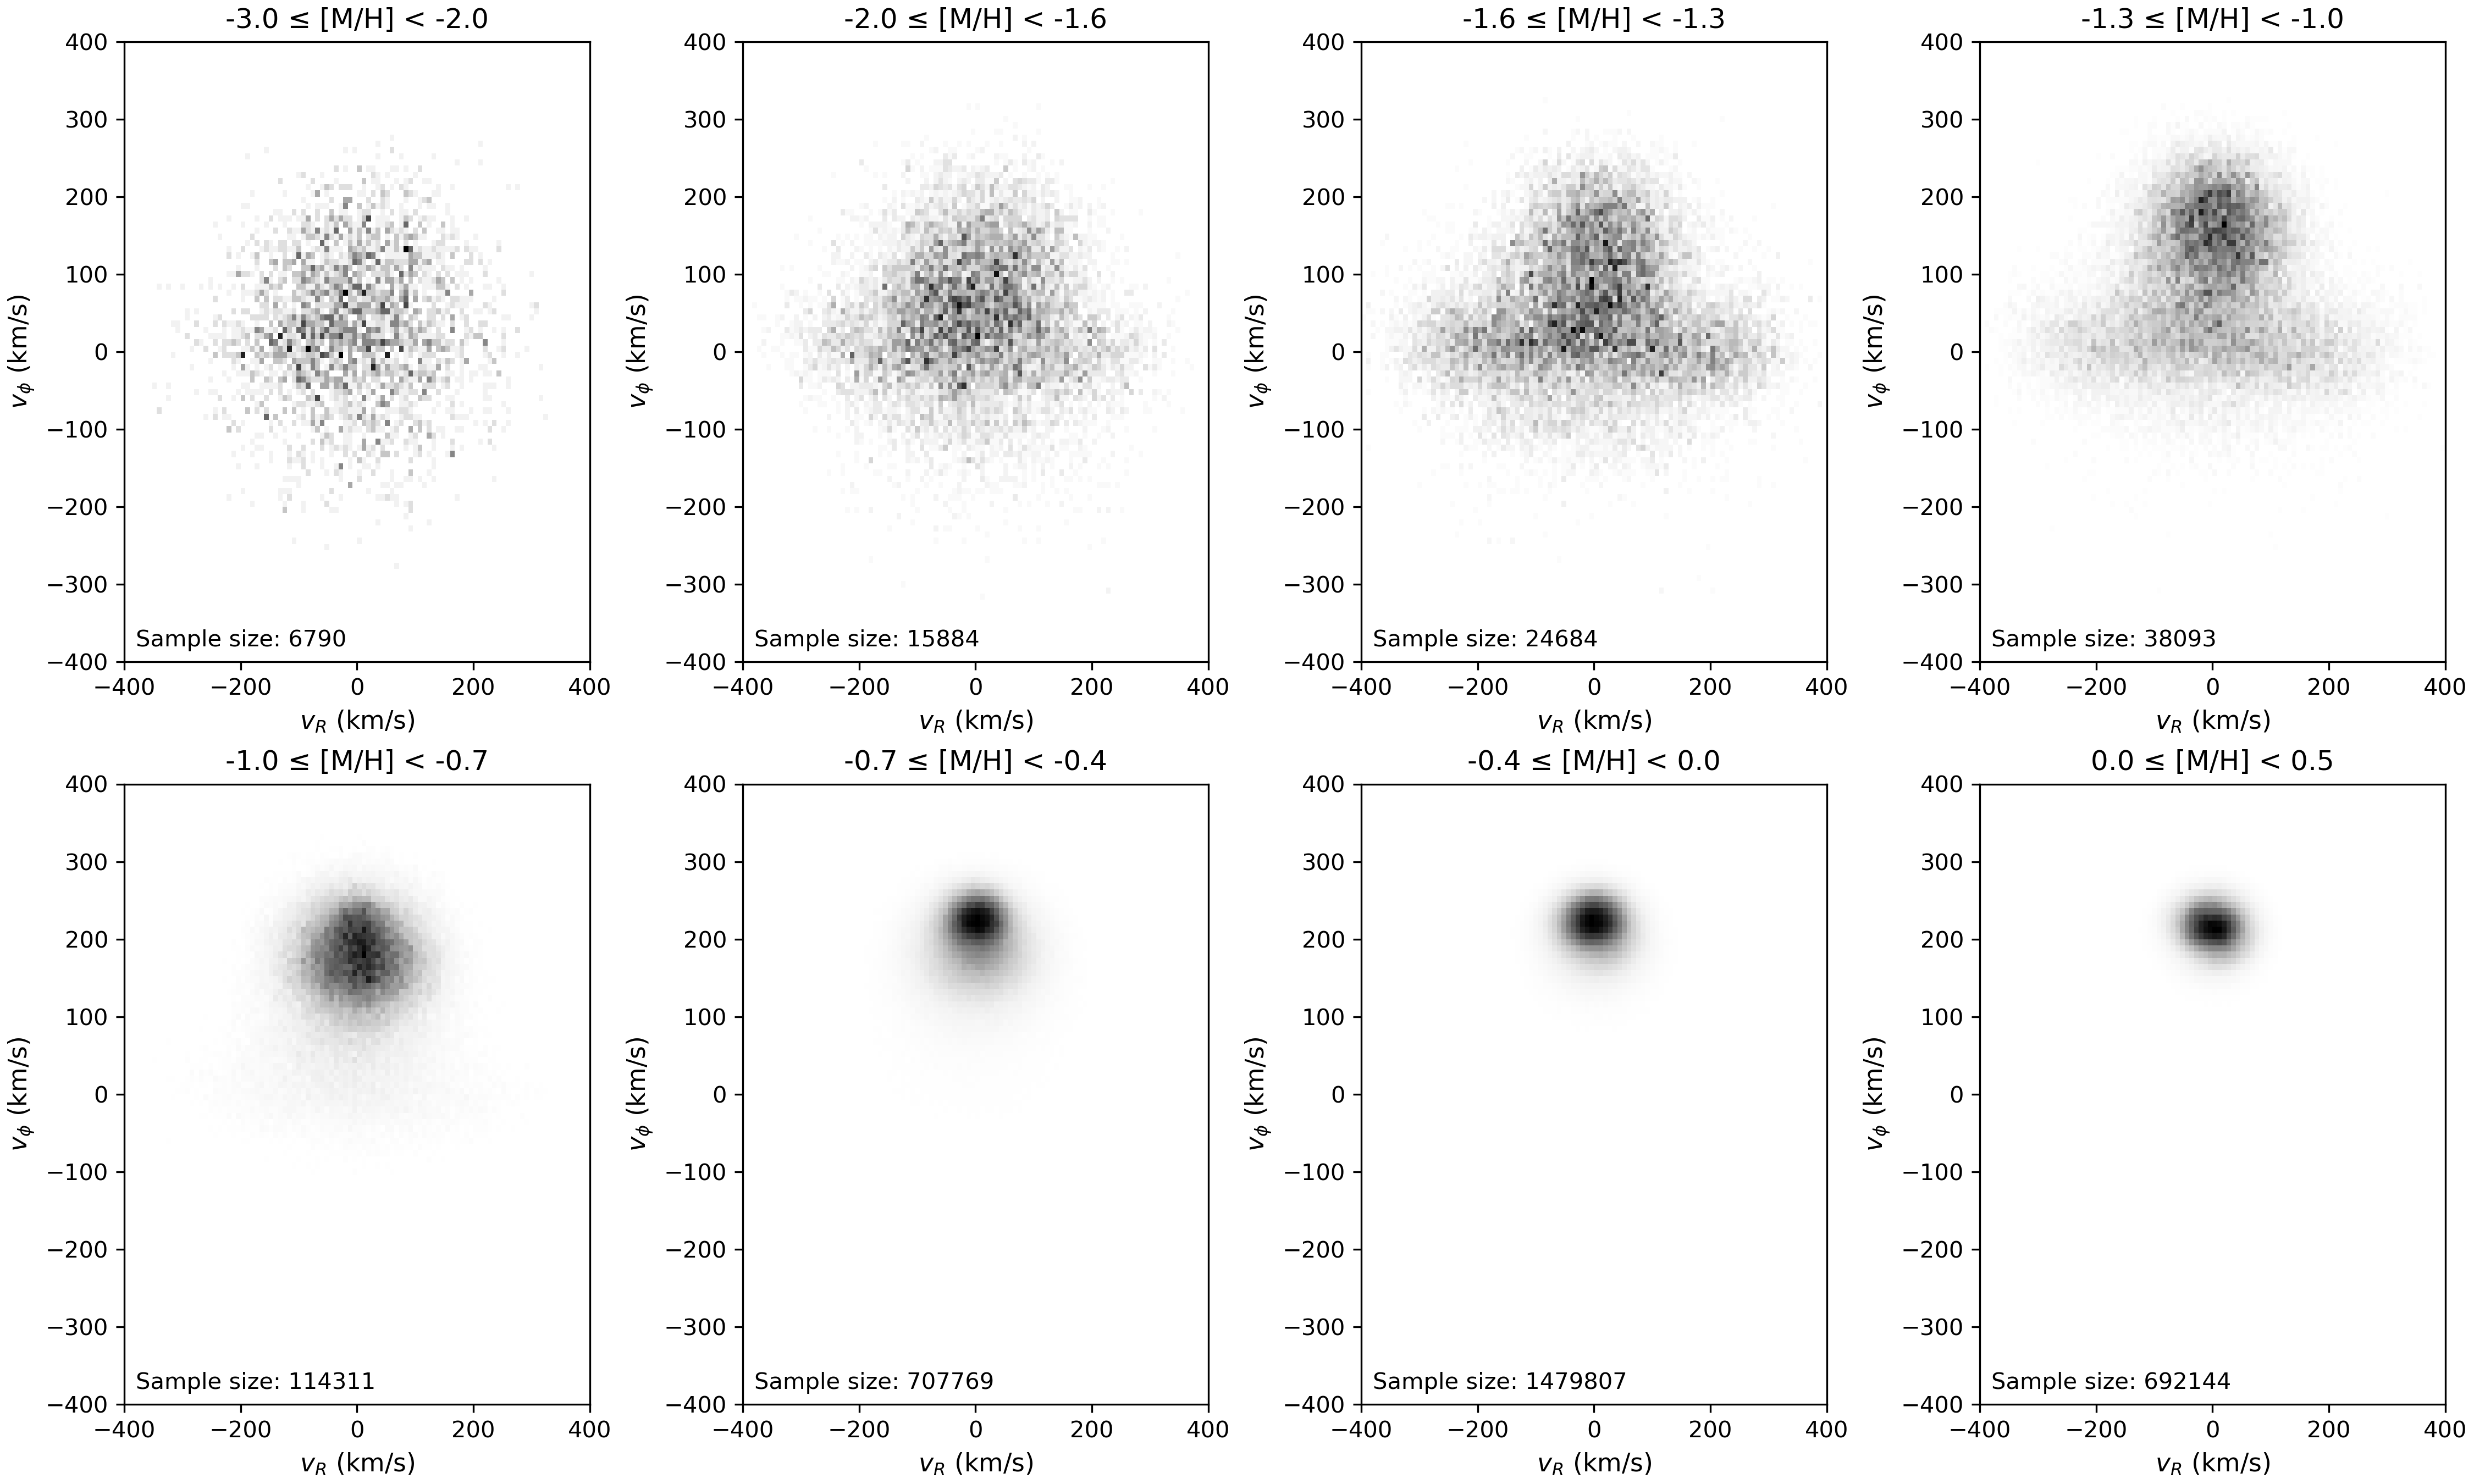
\includegraphics[width=\textwidth]
                   {../figures/vphi_metallicity_histograms.png}
  \caption{Galactocentric velocity distributions as a function of metallicity.
           Each panel shows the column–normalised density of stars in the
           $v_R$–$v_\phi$ plane for the metallicity interval printed at the
           top. With increasing metallicity the distribution contracts in both
           directions—signalling lower velocity dispersion—while the bulk
           of stars moves upward to larger prograde azimuthal velocity.
           }
  \label{fig:vRvphi_bins}
\end{figure}


\begin{figure}[h]
  \centering
  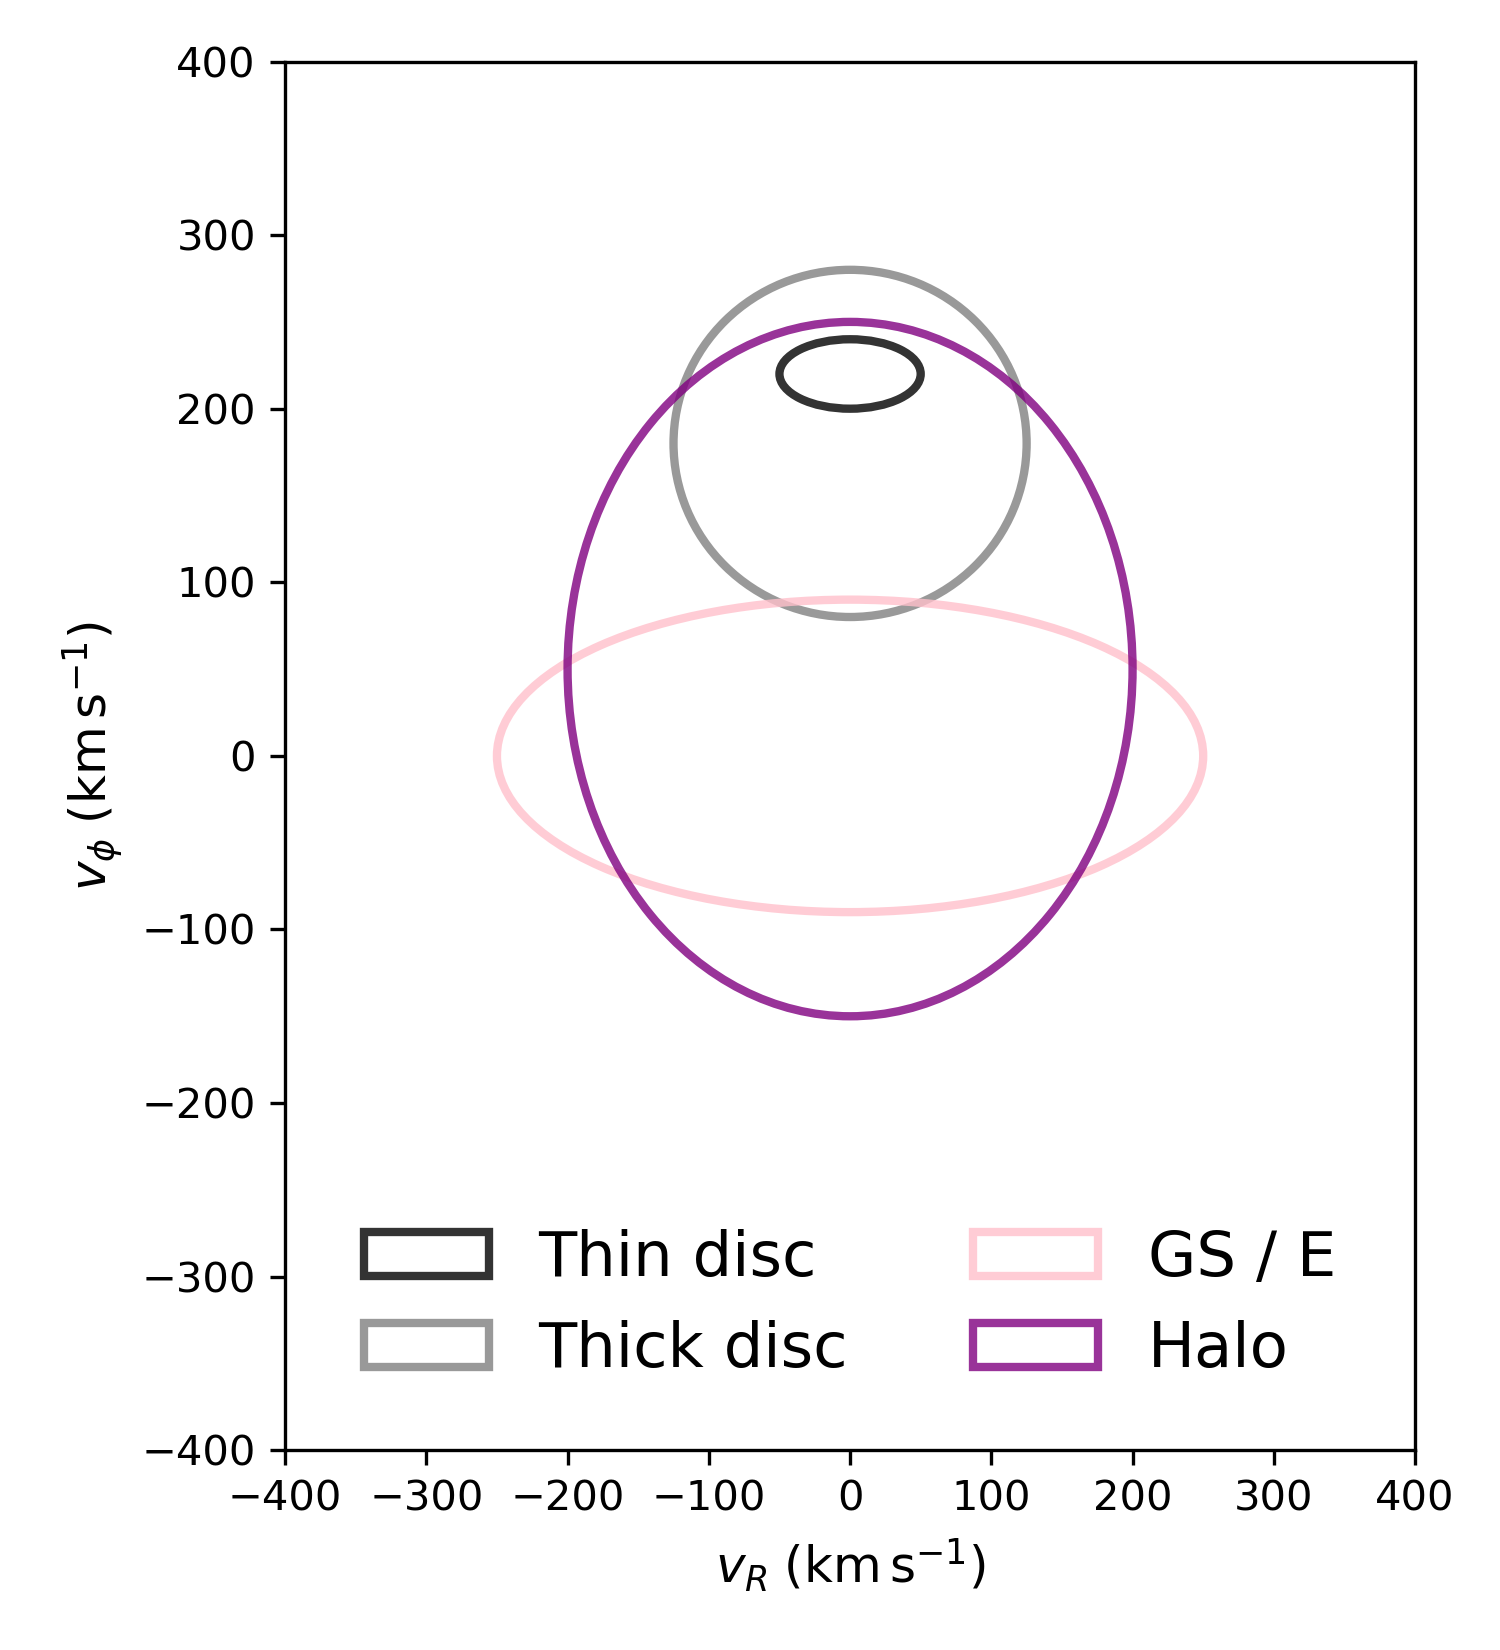
\includegraphics[width=0.3\columnwidth]
                   {../figures/reference_velocity_ellipses.png}
  \caption{Ellipses mark the approximate extent of the thin disc
           (\textcolor{black}{black}), thick disc (\textcolor{gray}{grey}),
           Gaia–Sausage/Enceladus debris (\textcolor{pink}{pink}) and the
           pressure-supported stellar halo (\textcolor{purple}{purple}).
           The figure serves as a visual key for interpreting the data panels
           in Fig.~\ref{fig:vRvphi_bins}.}
  \label{fig:ref_ellipses}
\end{figure}

As illustrated in Fig.~\ref{fig:vRvphi_bins}, stars richer than
${\rm[M/H]}\!\sim\!-1.0$ occupy the top of the $v_R$–$v_\phi$ plane,
clustering near the thin– and thick-disc ellipses in
Fig.~\ref{fig:ref_ellipses}.  Their large prograde azimuthal velocity
($v_\phi\!\gtrsim\!180$ km s$^{-1}$) and small radial dispersion
indicate rotation-dominated, dynamically cold orbits.
Below ${\rm[M/H]}\simeq-1.0$ the distribution broadens and
drops toward $v_\phi\!\approx\!0$, signalling a transition to
pressure-supported kinematics characteristic of the stellar halo and
the radial Gaia–Sausage/Enceladus debris.  At the lowest
metallicities (${\rm[M/H]}\lesssim-1.5$) the contours are nearly
isotropic with only a mild prograde bias, and the distinct disc
sequence seen at higher metallicity has vanished.  Hence, any
rotation-supported very-metal-poor disc must contribute at most a
small fraction of the population—an issue we quantify in
following analysis





\section{Methodology}
Details of your methodology.

\subsection{Extreme Deconvolution}
Discussion of XD.

\section{Results}
What you found.

\section{Extension direction}

\section{Conclusion}
Summary of your findings.



\newpage
\bibliographystyle{abbrvnat}
\bibliography{references}




\end{document}
